\chapter{事务}

\begin{definition}[事务]
  事务是由一系列操作序列构成的执行单元, 这些操作
要么都做, 要么都不做, 是一个不可分割的工作单位.
\end{definition}

\section{SQL中的事务}

\begin{enumerate}
    \item 事务以\verb|begin transaction|开始, 以\verb|commit transaction|或\verb|rollback transaction|结束.
    \item \verb|commit transaction|表示提交, 事务正常结束.
    \item \verb|rollback transaction|表示事务非正常结束, 撤消事务已做的操作, 回滚到事务开始时状态.
\end{enumerate}

\begin{lstlisting}[language=SQL]
create table accounts ( userId char(4) primary key,
                        amounts int check ( amounts >= 0 ) ) ;
insert into accounts values ('A',1000), ('B', 2000);
set transaction isolation level read committed;
start transaction;
update accounts set amounts = amounts - 50 where userId='A';
update accounts set amounts = amounts + 50 where userId='B';
commit;
\end{lstlisting}

事务的执行模式:
\begin{enumerate}
    \item 显式事务: 以begin transaction开始, 以commit或rollback结束.
    \item 隐含事务(SQL Server): 事务自动开始, 直到遇到commit或rollback时结束.
    
    \verb+set implicit_transactions {ON | OFF}+.
    \item 自动事务(MySQL): 每个数据操作语句作为一个事务. \verb+set autocommit = {1 | 0}+.
\end{enumerate}

事务中的错误检查:
\begin{enumerate}
    \item SQL Server: \verb|set XACT_ABORT ON|.
    \item MySQL: \verb|declare exit handler for SQLEXCEPTION rollback|.
\end{enumerate}

\subsection{事务基本特性ACID}

\begin{enumerate}
    \item 原子性(Atomicity).
    \begin{enumerate}
        \item 事务中包含的所有操作要么全做, 要么全不做.
        \item 原子性由\textcolor{red}{恢复机制}实现.
    \end{enumerate}
    \item 一致性(Consistency).
    \begin{enumerate}
        \item 事务的隔离执行必须保证数据库的一致性.
        \item 事务开始前, 数据库处于一致性状态; 事务结束后, 数据库必须仍处于一致性状态.
        \item 数据库一致性状态由\textcolor{red}{用户}来负责.
    \end{enumerate}
    \item 隔离性(Isolation).
    \begin{enumerate}
        \item 系统必须保证事务不受其它并发执行事务的影响.
        \item 对任何一对事务$T_1,T_2$, 在$T_1$看来, $T_2$要么在$T_1$开始之前已经结束, 要么在$T_1$完成之后再开始执行: $T_1\to T_2 \text{ or } T_2\to T_1$.
        \item 隔离性通过\textcolor{red}{并发机制}实现.
    \end{enumerate}
    \item 持久性(Durability).
    \begin{enumerate}
        \item 一个事务一旦提交之后, 它对数据库的影响必须是永久的.
        \item 系统发生故障不能改变事务的持久性.
        \item 持久性通过\textcolor{red}{恢复机制}实现.
    \end{enumerate}
\end{enumerate}

\begin{figure}[H]
    \centering
    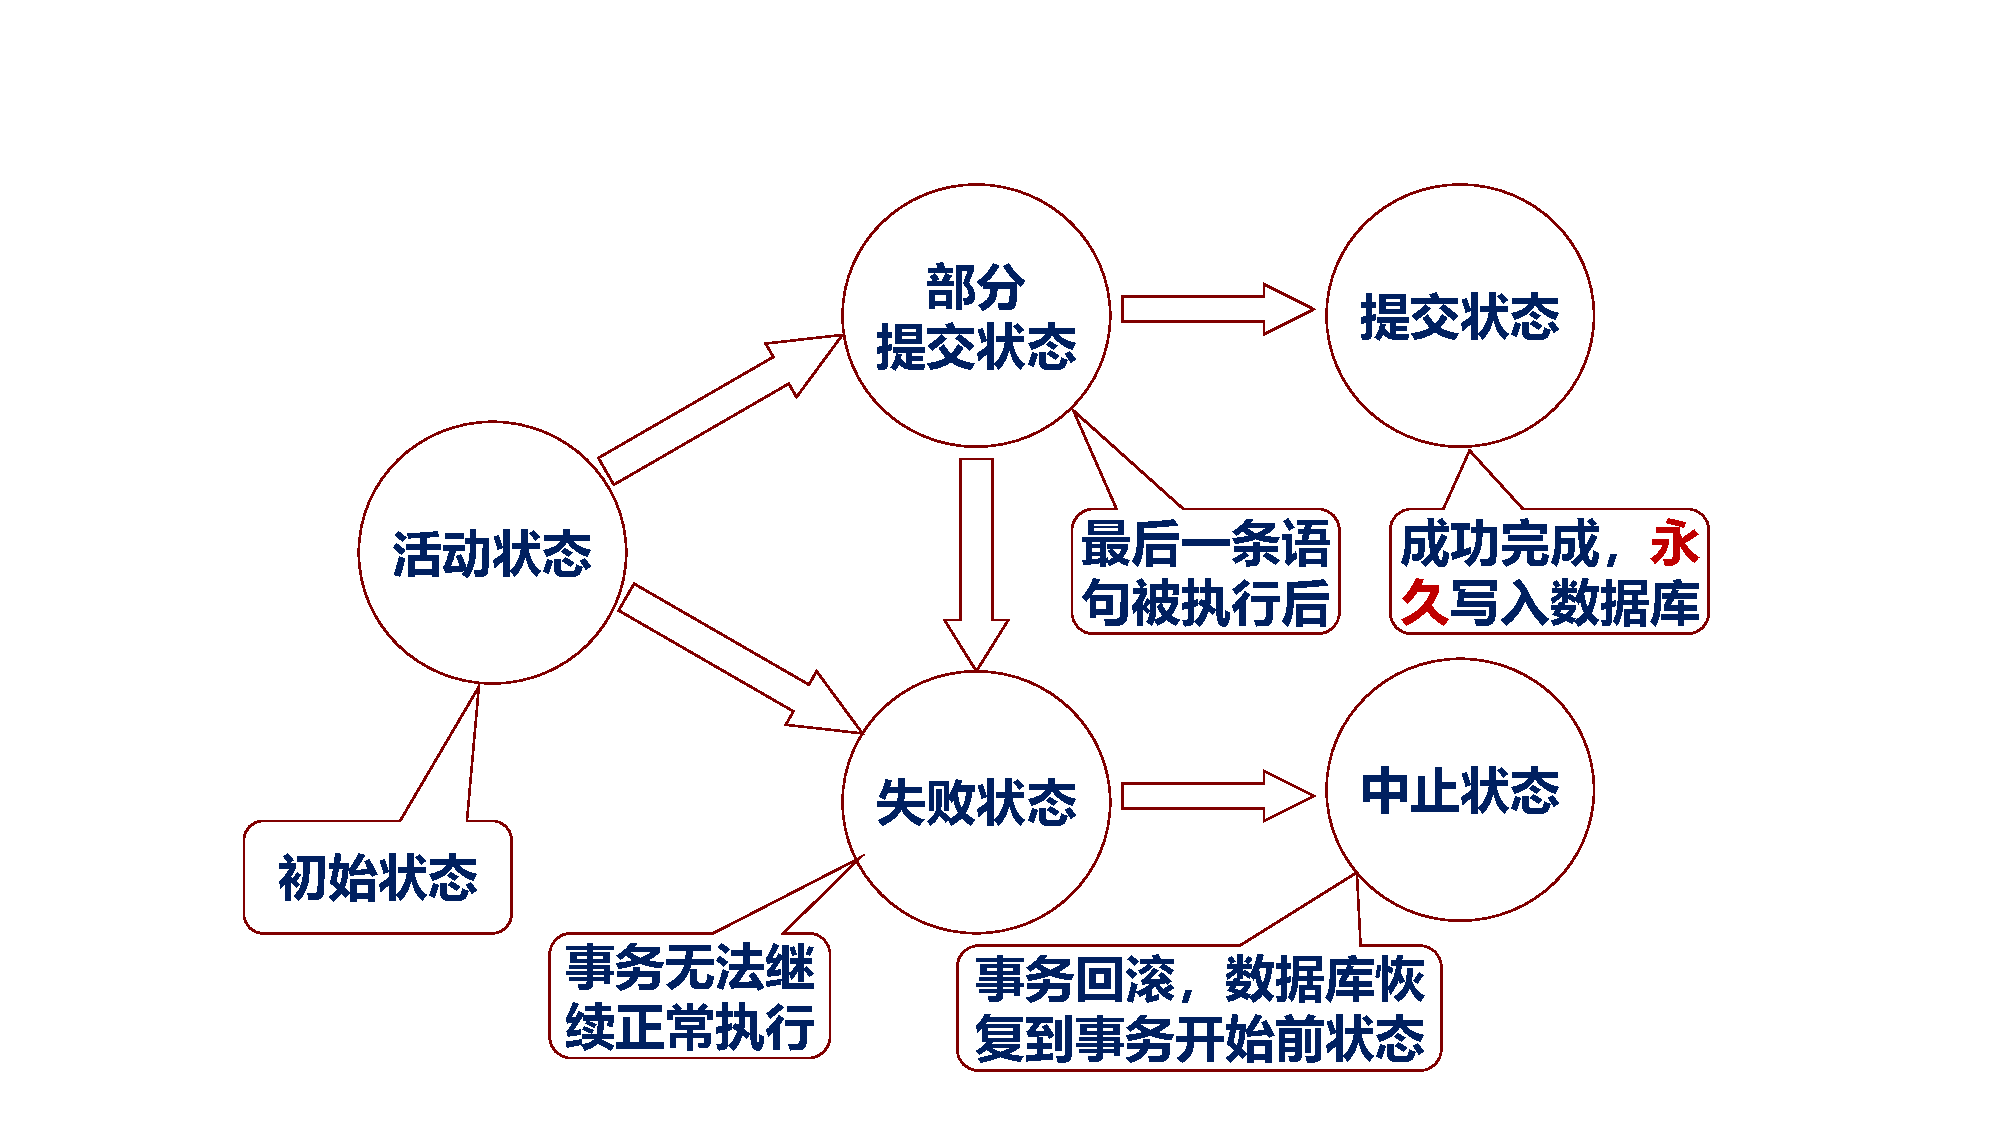
\includegraphics[width=.6\textwidth]{./figure/事务生命周期.pdf}
    \caption{事务生命周期图}
\end{figure}

\section{事务调度}

\begin{definition}[调度]
  事务的执行顺序称为一个调度, 表示事务的指令在系统中执行的时间顺序.

  一组事务的调度必须保证:
  \begin{enumerate}
      \item 包含了所有事务的操作指令.
      \item 一个事务中指令的顺序必须保持不变.
  \end{enumerate}
\end{definition}

\begin{definition}[串行调度]
  \begin{enumerate}
      \item 在串行调度中, 属于同一事务的指令紧挨在一起.
      \item 对于有$n$个事务的事务组, 可以有$n!$个有效调度.
  \end{enumerate}
\end{definition}

\begin{definition}[并行调度]
  \begin{enumerate}
      \item 在并行调度中, 来自不同事务的指令可以交叉执行.
      \item 当并行调度等价于某个串行调度时, 则称它是正确的.
  \end{enumerate}
\end{definition}

\begin{example}
  $n$个事务, $T_i$有$k_i$条指令, 则可能的并发调度有多少个?

  调度数为:
  \begin{align*}
      \frac{\left(\sum_{i=1}^{n}k_i\right)!}{\prod_{i=1}^n k_i!}.
  \end{align*}
\end{example}

\begin{definition}[可恢复调度]
  对于每对事务$T_i$与$T_j$, 如果$T_j$读取了$T_i$所写的数据, 则$T_i$必须先于$T_j$提交.
  \begin{enumerate}
      \item 一个事务失败了, 应该能够撤消该事务对数据库的影响.
      \item 如果有其它事务读取了失败事务写入的数据, 则该事务应该撤消.
  \end{enumerate}
\end{definition}

\begin{definition}[级联调度]
  由于一个事务故障而导致一系列事务回滚.
\end{definition}

\begin{definition}[无级连调度]
  对于任意两个事务$T_i$和$T_j$, 如果$T_j$读取了$T_i$写入的数据项, 则$T_i$的提交操作必须在$T_j$的操作之前完成.

  无级联调度必是可恢复调度.
\end{definition}

\subsection{并发调度中的不一致现象}

丢失修改: 写写不一致. 两个事务$T_1$和$T_2$读入同一数据并修改, 
$T_1$提交的结果破坏了$T_2$提交的结果, 导致$T_2$的修改丢失.

读脏数据: 写读不一致. 事务$T_1$修改某一数据并将其写回磁盘, 
事务$T_2$读取同一数据. 
此后$T_1$由于某种原因被撤消, 其已修改过的数据恢复原值, 
造成$T_2$读到的数据与数据库中数据不一致, 则$T_2$读到的就是脏数据.

不能重复读: 读写不一致. 事务$T_2$读取某一数据后, 事务$T_1$对其做了修改, 
当$T_2$再次读取该数据时, 得到与前次不同的值.

发生幻象(Phantom): 插读不一致. 事务$T_2$按一定条件读取某些数据后, 
事务$T_1$插入一些满足这些条件的数据, 
当$T_2$再次按相同条件读取数据时, 发现多了一些记录.

解决方案:
\begin{enumerate}
    \item 丢失修改: 两个事务不能同时修改同一数据项.
    \item 读脏数据: 只能读取已提交数据。
    \item 不能重复读: 两次读取之间不能有其他事务修改该数据项.
    \item 幻象: 两次读取不能插入.
\end{enumerate}

\section{事务隔离性级别}

\begin{enumerate}
    \item read uncommitted: 允许读取未提交的记录.
    \item read committed: 只允许读取已提交的记录, 但不要求可重复读.
    \item repeatable read: 只允许读取已提交记录, 并且一个事务对同一记录的两次读取之间, 其它事务不能对该记录进行更新.
    \item serializable: 调度的执行必须等价于串行调度.
\end{enumerate}

\begin{table}[H]
  \centering
  \begin{tabular}{|c|c|c|c|c|}
    \hline
    \textbf{隔离性级别} & \textbf{读脏数据} & \textbf{不能重复读} & \textbf{幻象} & \textbf{丢失修改} \\ \hline
    Read uncommitted & 是 & 是 & 是 & 是 \\ \hline
    Read committed & 否 & 是 & 是 & 是 \\ \hline
    Repeatable read & 否 & 否 & 是 & 否 \\ \hline
    Serializable & 否 & 否 & 否 & 否 \\ \hline
  \end{tabular}
  \caption{事务隔离性级别}
\end{table}

\section{快照隔离}

快照隔离(Snapshot Isolation, SI)的基本思想: 多版本+回滚.
\begin{itemize}
  \item 对数据库的写发生在提交时, 形成数据项的一个提交版本(快照).
  \item 执行时间和访问数据项有交叠的写事务之间会产生冲突, 先提交者赢.
  \item 读操作访问该读事务开始那一刻的数据项最新版本, 读写相互不会阻塞.
\end{itemize}

\begin{figure}[H]
    \centering
    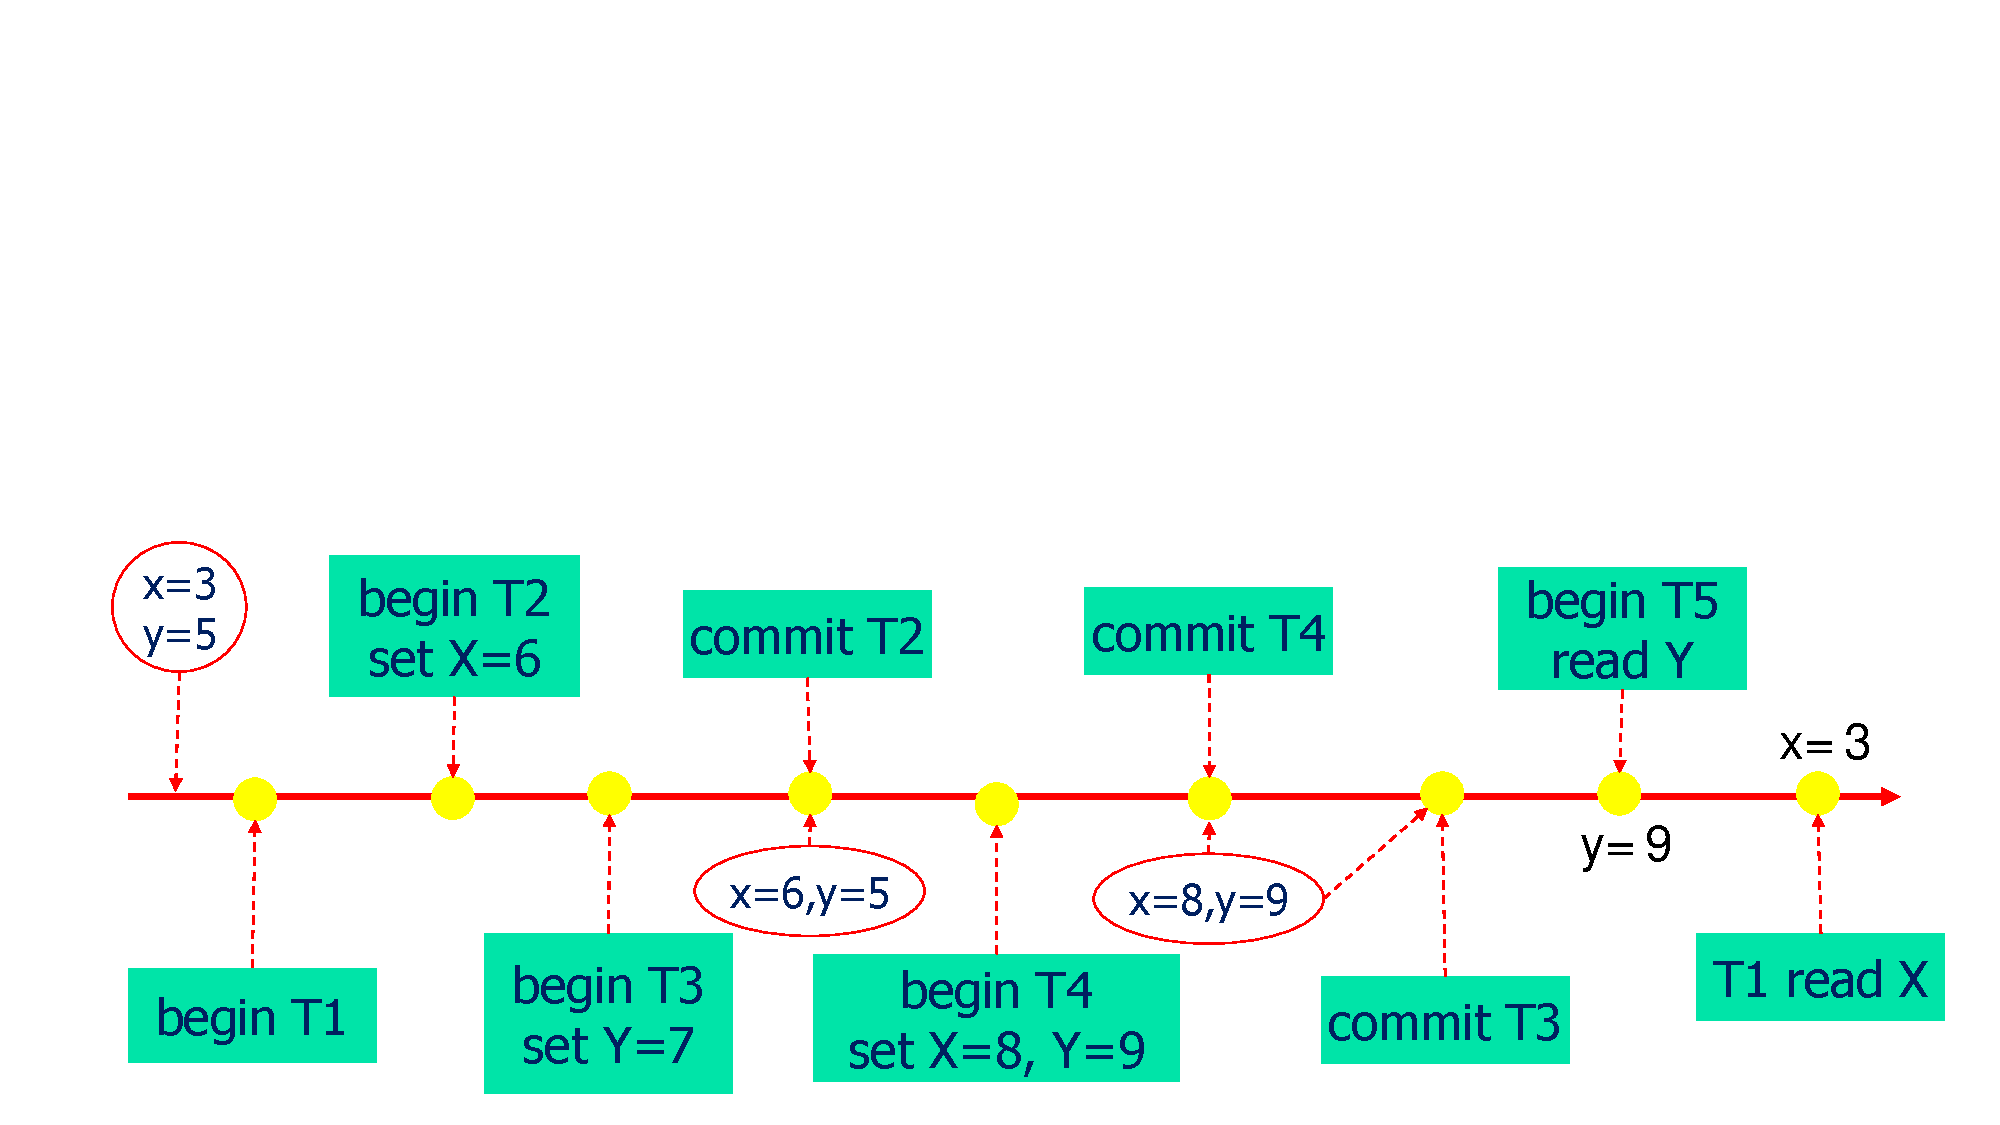
\includegraphics[width=.6\textwidth]{./figure/快照隔离.pdf}
    \caption{快照隔离}
\end{figure}

快照隔离中有不一致的现象.
\begin{example}
  现在有一致性要求: $X+Y\ge 0$, 下面的调度会导致一致性被违反.
  \begin{figure}[H]
      \centering
      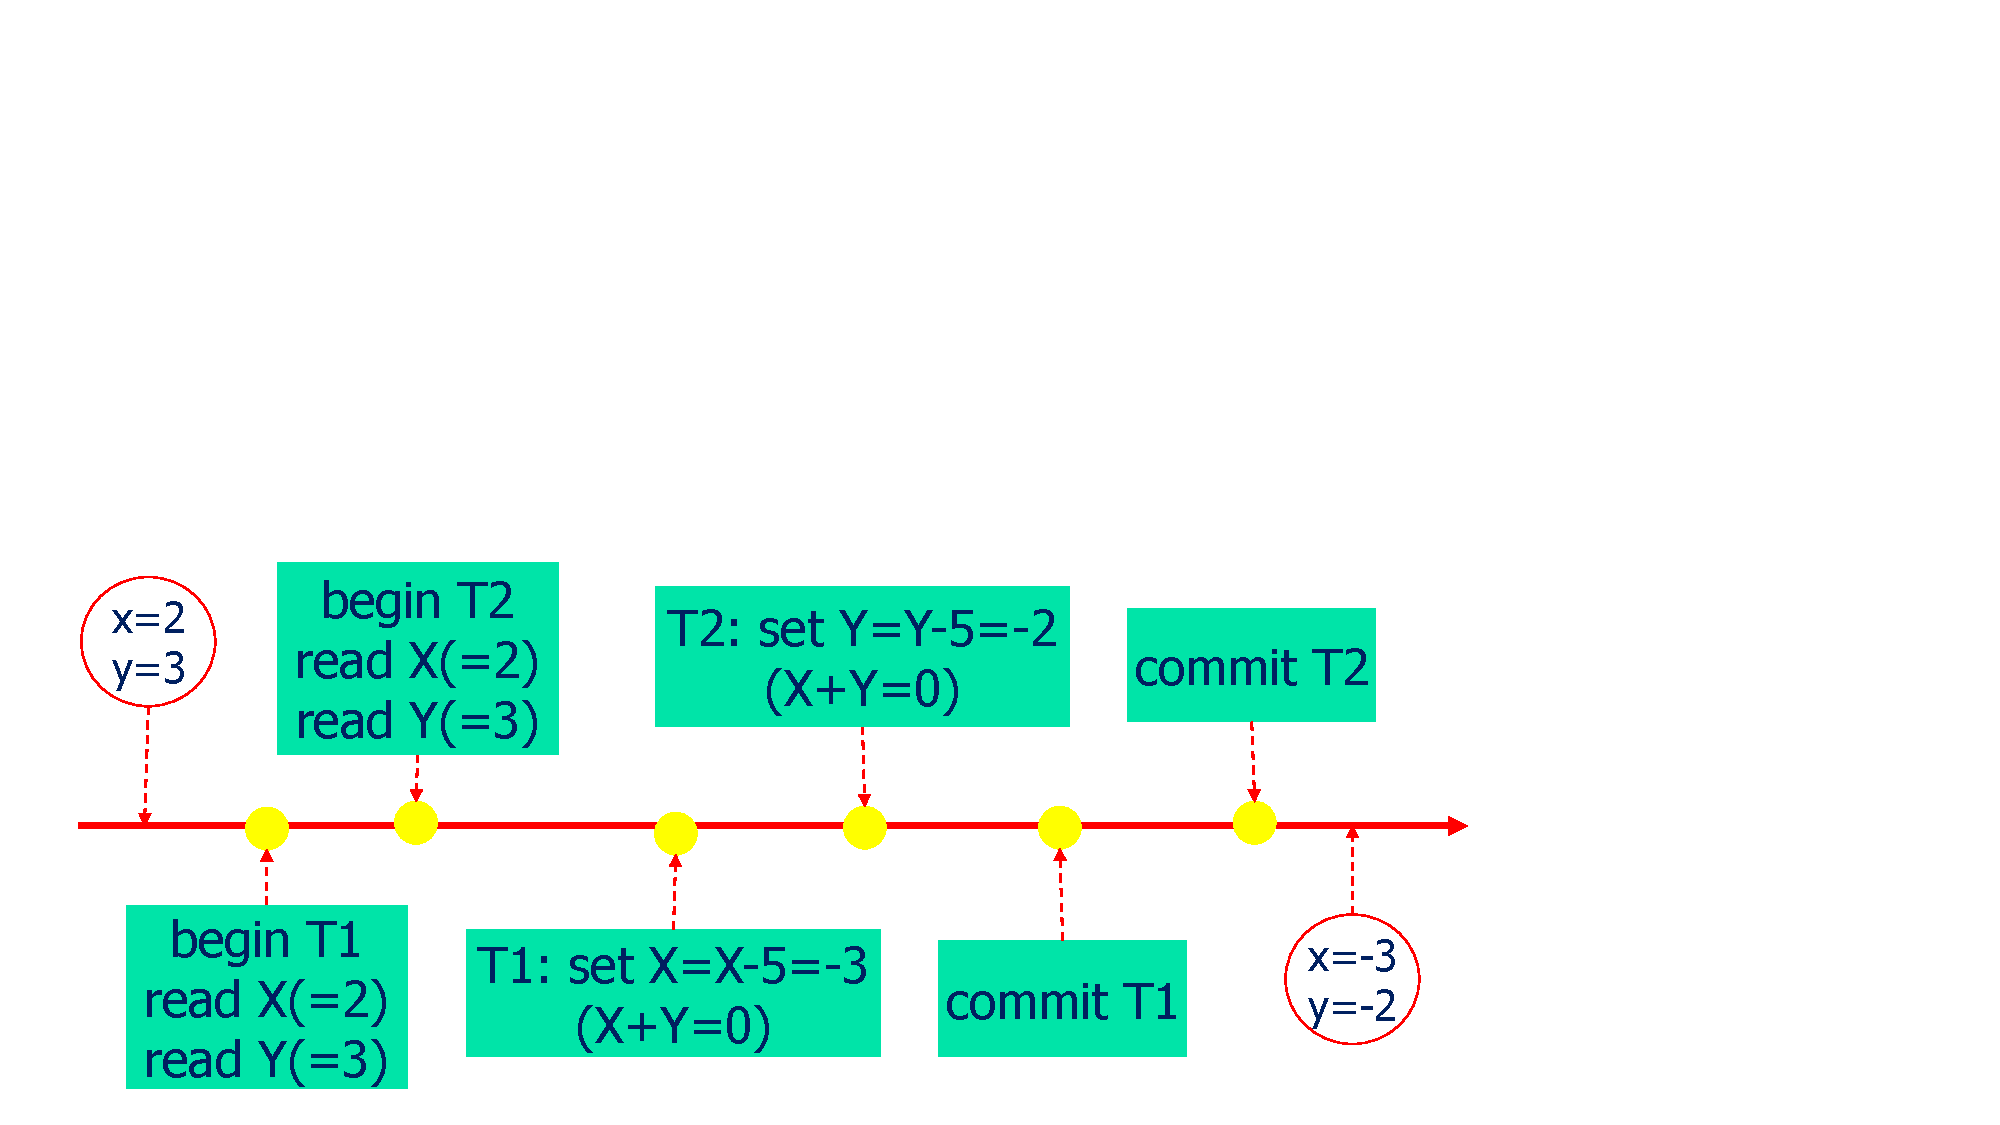
\includegraphics[width=.5\textwidth]{./figure/快照隔离不一致.pdf}
      \caption{快照隔离中的不一致现象}
  \end{figure}
\end{example}

SQL Server中的快照隔离:
\begin{enumerate}
    \item 事务级快照隔离: 读取操作得到数据项在事务开始时刻最近的已提交版本. 通过回滚解决冲突更新操作.
    \item 语句级快照隔离(Read Commited SI, RCSI): 读取操作得到数据项在语句开始时刻最近的已提交版本. 通过阻塞解决冲突更新操作.
\end{enumerate}

\section{事务可串行化判定}

事务可串行化判定, 如何判定两个调度是等价的?
\begin{itemize}
  \item 冲突可串行化: 冲突指令. \textit{微观角度: 是否可以交换两个相邻指令?}
  \item 视图可串行化: 从读一致性. \textit{宏观视角: 如何保证每个事务在两个调度中是相同的?}
\end{itemize}

\subsection{冲突可串行化}

考虑一个调度$S$中的两条连续指令(仅限于read和write)$I_j$和$I_j$, 分别属于事务$T_i$和$T_j$.
\begin{enumerate}
    \item $I_i=\text{read}(Q), I_j=\text{read}(Q)$.
    \item $I_i=\text{read}(Q), I_j=\text{write}(Q)$.
    \item $I_i=\text{write}(Q), I_j=\text{read}(Q)$.
    \item $I_i=\text{write}(Q), I_j=\text{write}(Q)$.
\end{enumerate}

只有上面的情况1可交换.

\begin{definition}[冲突指令]
  两条指令是不同事务在\textcolor{red}{相同数据项}上的操作, 并且其中至少有一个是write指令.
\end{definition}

\begin{definition}[冲突等价]
  如果调度$S$可以经过交换一系列非冲突指令转换成调度$S'$, 则称调度$S$与$S'$是冲突等价的.
\end{definition}

\begin{definition}[冲突可串行化]
  当一个调度$S$与一个串行调度冲突等价时则称该调度是\textcolor{red}{冲突可串行化}的.
\end{definition}

\begin{definition}[优先图]
  调度$S$的优先图(Precedence Graph)是一个有向图$G=(V,E)$, $V$是顶点集,
  $E$是边集. 顶点集由所有参与调度的事务组成, 边集由满足下述条件之一的边$T_i\to T_j$组成:
  \begin{enumerate}
      \item 在$T_j$执行$\text{read}(Q)$之前, $T_i$执行$\text{write}(Q)$.
      \item 在$T_j$执行$\text{write}(Q)$之前, $T_i$执行$\text{read}(Q)$.
      \item 在$T_j$执行$\text{write}(Q)$之前, $T_i$执行$\text{write}(Q)$.
  \end{enumerate}
\end{definition}

\begin{theorem}
  如果优先图中存在边$T_i\to T_j$, 则在任何等价于$S$的串行调度$S'$中, $T_i$都必须出现在$T_j$之前.
\end{theorem}

\begin{lemma}[有向无环图一定有一个入度为0的节点]\label{lemma:DAG}
  有向无环图一定有一个入度为0的节点.
\end{lemma}
\begin{proof}
  我们称入度为0的节点为源点.

  假设$n$个顶点的有向无环图没有源点, 对于顶点$v_{i1}$, 
  由于其不是源点, 那么一定存在一个节点$v_{i2}$, 
  且从$v_{i2}$到$v_{i1}$有一条有向边.
  依此类推, 可以得到一条路径: $v_{ik}\to \dots v_{i2}\to v_{i1}$.
  \begin{itemize}
    \item 对于$v_{ik}$的入边的起始节点$v_{i,k+1}$, 如果$v_{i,k+1}\in\{v_{i1}, v_{i2},\dots v_{ik}\}$, 构成了环, 矛盾.
    \item 如果$v_{i,k+1}\not\in\{v_{i1}, v_{i2},\dots v_{ik}\}$, 由于顶点数量$n$是有限的, 那么可以一直扩展此路径, 直到所有顶点都包含在此路径中, 即$v_{in}\to \dots v_{i2}\to v_{i1}$.
    此时该路径的起始顶点$v_{in}$由于不是源点, 一定有另外一个顶点$v_{im}$可直达$v_{in}$,
    而$v_{im}\in\{v_{i1},v_{i2},\dots,v_{in}\}$, 则也构成回路, 矛盾.
  \end{itemize}
  综上所述, 可证明一个有向无环图中至少有一个源点.
\end{proof}

\begin{theorem}
  如果调度$S$的优先图中有环, 则$S$是非冲突可串行化的;
  如果图中无环, 则是冲突可串行化的.
\end{theorem}

\begin{proof}
  首先, 根据引理\ref{lemma:DAG}, 考虑到有向无环图中一定存在一个节点入度为0. 然后计算出拓扑排序即可.
\end{proof}

与冲突可串行化等价的串行顺序 = 拓扑排序.

\subsection{视图可串行化}

\begin{definition}[视图等价]
  考虑关于某个事务集的两个调度$S,S'$, 若调度$S,S'$满足以下条件, 则称它们是\textcolor{red}{视图等价}的:
  \begin{enumerate}
      \item $[\![\text{数据库初值}]\!]\overset{S}{\to}r_i(Q)\land [\![\text{数据库初值}]\!]\overset{S'}{\to}r_i(Q)$.
      \item $[\![w_j(Q)]\!]\overset{S}{\to}r_i(Q)\land [\![w_j(Q)]\!]\overset{S'}{\to}r_i(Q)$.
      \item $w_i(Q)\overset{S}{\to}[\![\text{数据库终值}]\!]\land w_i(Q)\overset{S'}{\to}[\![\text{数据库终值}]\!]$.
  \end{enumerate}
\end{definition}
\begin{remark}
  条件1和2保证从读一致性, 条件3保证两个调度得到最终相同的系统状态.
\end{remark}

\begin{figure}[H]
    \centering
    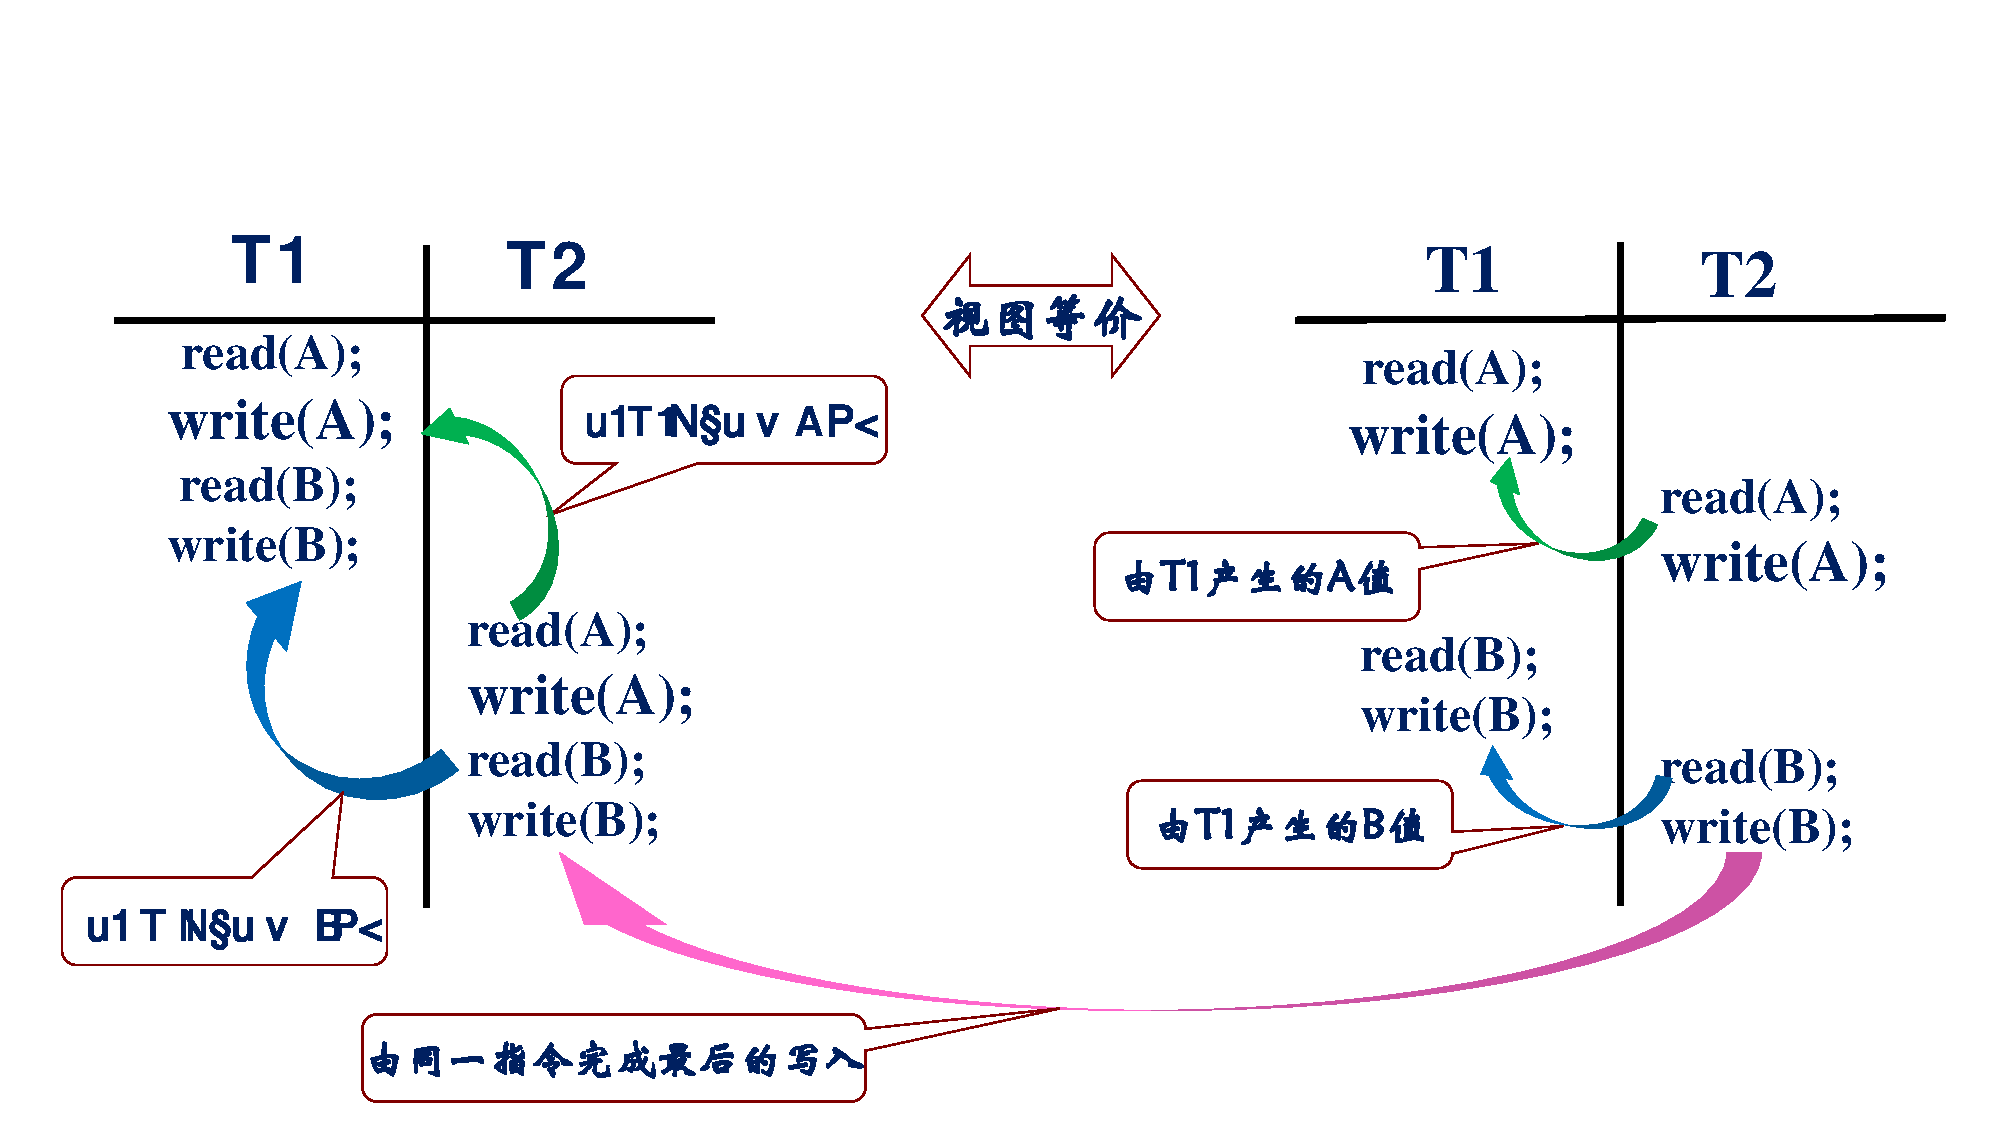
\includegraphics[width=.7\textwidth]{./figure/视图等价.pdf}
    \caption{视图等价}
\end{figure}


\begin{definition}[视图可串行化]
  如果某个调度视图等价于一个串行调度, 则称该调度是
  \textcolor{red}{视图可串行化}的.
\end{definition}

\begin{corollary}
  冲突可串行化调度一定是视图可串行化的.
\end{corollary}

\begin{corollary}
  存在视图可串行化但非冲突可串行化的调度.
\end{corollary}

盲目写操作: write之前并不执行read操作.

无用的写操作: 被覆盖掉的写操作.

带标记的优先图的构造:
设调度 $ S = \{ T_1, T_2, \ldots, T_n \} $, 构造两个虚事务 $ T_b, T_f $, 
其中 $ T_b $ 为 $ S $ 中所有 $ \text{write}(Q) $ 操作, 
$ T_f $ 为 $ S $ 中所有 $ \text{read}(Q) $ 操作. 
在调度 $ S $ 的开头插入 $ T_b $, 在调度 $ S $ 的末尾插入 $ T_f $, 得到新的调度 $ S' $.
\begin{enumerate}
    \item 如果 $ T_j $ 读取 $ T_i $ 写入的数据项的值,则加入边 $ T_i \overset{0}{\to} T_j $.
    \item 如果在优先图中不存在从 $ T_i $ 到 $ T_f $ 的通路, 则 $ T_i $ 是无用事务, 将其删除.
    \item 对于每个数据项 $ Q $, 如果 $ T_j $ 读取 $ T_i $ 写入的 $ Q $ 值, $ T_k $ 执行 $ \text{write}(Q) $ 且 $ T_k \neq T_b $, 则: \textit{其实在考虑$T_i \overset{0}{\to} T_j$之间插入$T_k$.}
    \begin{enumerate}
        \item 如果 $ T_i = T_b $ 且 $ T_j \neq T_f $, 考虑 $ T_k $ 在优先图中的位置: 插入$T_j\overset{0}{\to}T_k$.
        \item 如果$T_i\neq T_b$且$T_j=T_f$, 考虑$T_k$在优先图中的位置: 插入$T_k\overset{0}{\to} T_i$.
        \item 如果$T_i\neq T_b$且$T_j\neq T_f$, 考虑$T_k$在优先图中的位置: $T_k\overset{p}{\to} T_i$和$T_j\overset{p}{\to} T_k$. 其中$p$是一个唯一的, 在前面边的标记中未曾用过的大于0的整数.
        \textit{这实际上是说这两条边二选一.}
    \end{enumerate}
\end{enumerate}
标号为0的边组成底图, 标号为$p$的取出一条可以形成两张图, 判定是否有环.

\begin{theorem}[视图可串行化判定准则]
  只要有一个优先图无环, 则调度是视图可串行化的.
\end{theorem}

存在可串行化但非视图可串行化的调度:
\begin{figure}[H]
    \centering
    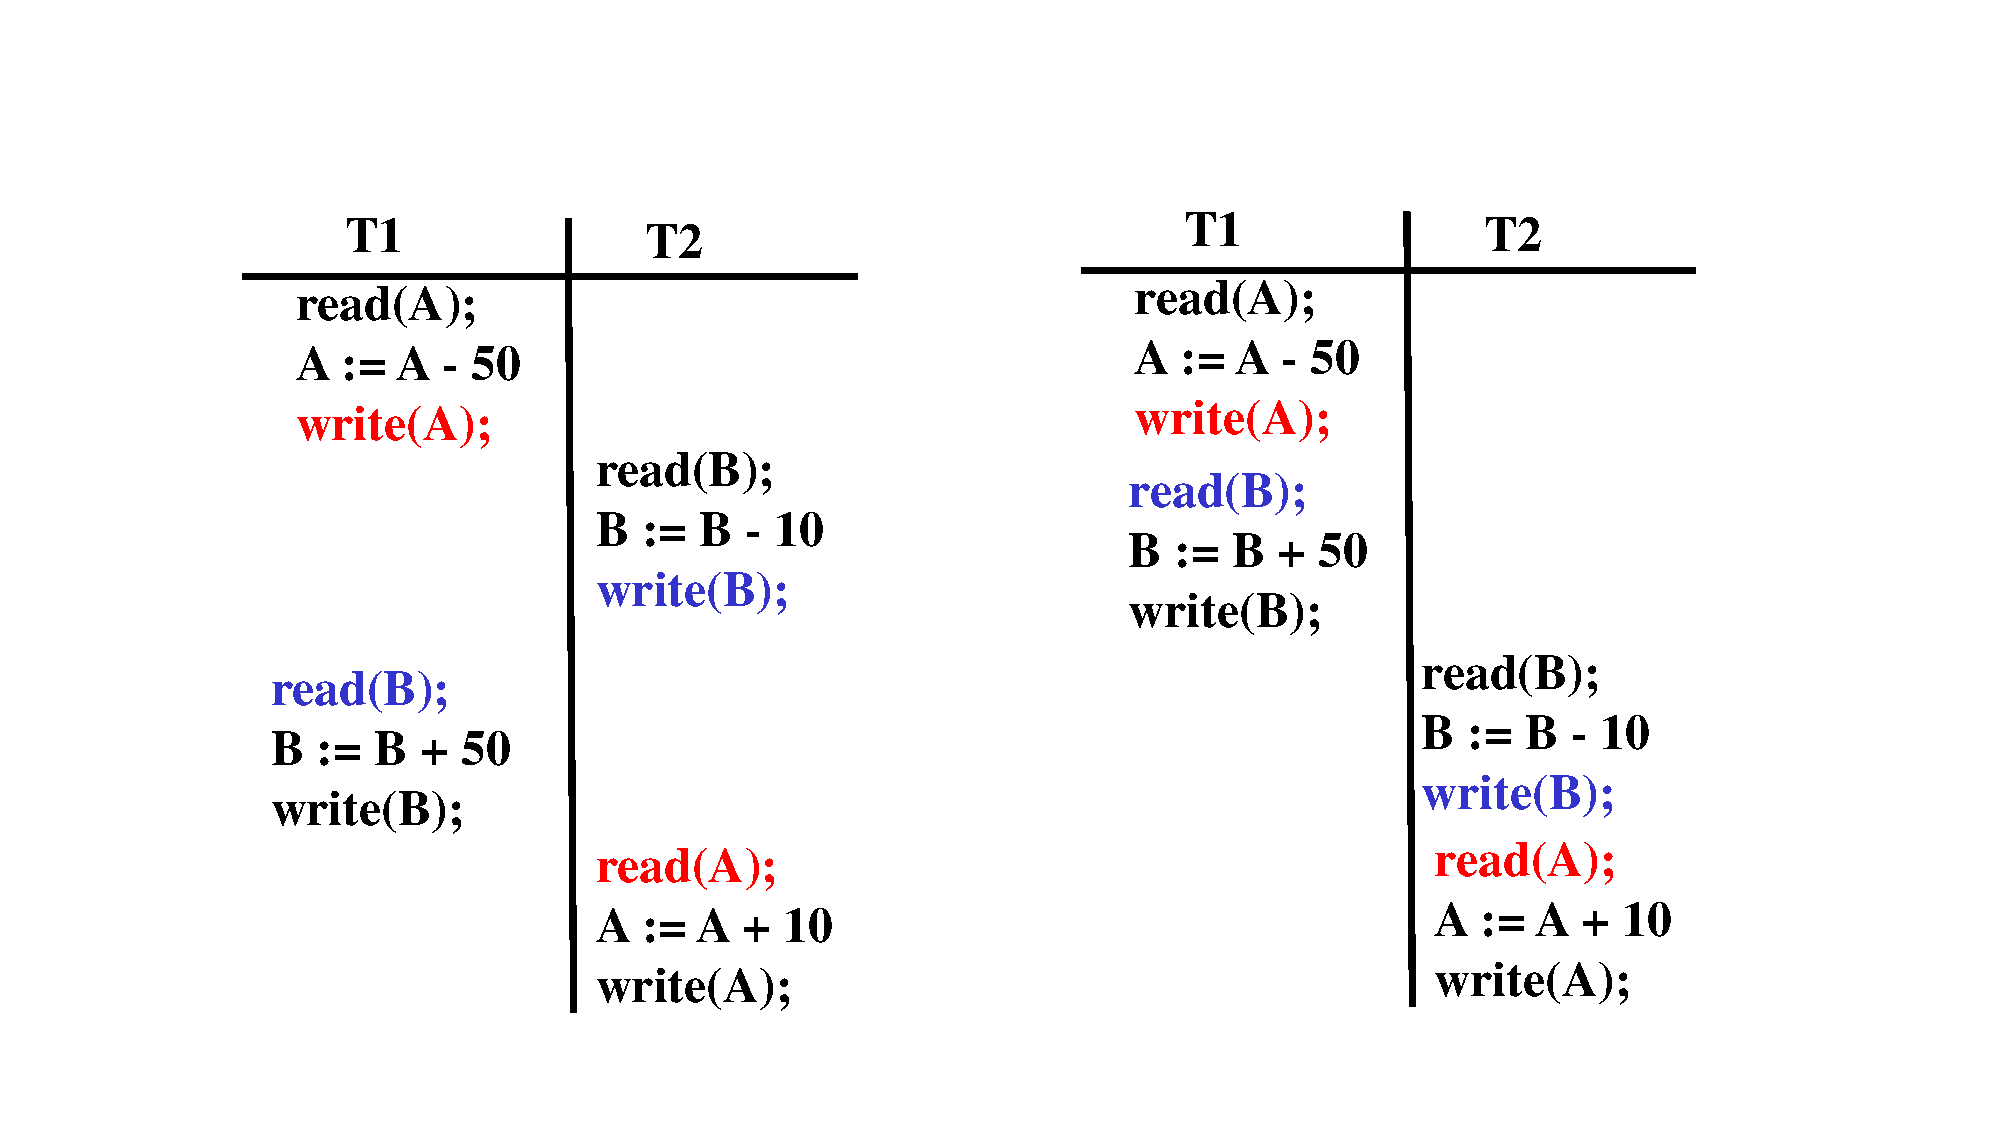
\includegraphics[width=.7\textwidth]{./figure/可串行化.pdf}
    \caption{可串行化但非视图可串行化的调度}
\end{figure}

\section{保存点}

平面事务: 一层结构\verb|begin transaction...commit|.

平面事务的缺点: 不能部分回滚.

需要部分回滚的场合:
\begin{enumerate}
    \item 非线性流程控制. 比如订票分段, 只需要回滚到没订上的那一段.
    \item 批量更新.
\end{enumerate}

解决方法: 保存点.
\begin{lstlisting}[language=SQL]
  begin
    S1;
    sp1 := create_savepoint();
    ...
    Sn;
    spn := create_savepoint();
    ...
    if (condition) rollback(spi);
    ...
  commit();
\end{lstlisting}

\begin{lstlisting}[language=SQL]
  start transaction;
  insert into test_savePoint values ('sp0');
  savepoint sp1;
  insert into test_savePoint values ('sp1');
  savepoint sp2;
  insert into test_savePoint values ('sp2');
  savepoint sp3;
  insert into test_savePoint values ('sp3');
  rollback to sp2;
  commit;
\end{lstlisting}